% ============================================================================
%  SECTION 3: THE PHILOSOPHY OF MACHINE MINDS
%  Prediction=Compression=Intelligence · The Platonic Representation Hypothesis
%  · The Chinese Room Revisited
% ============================================================================
\documentclass[aspectratio=169, 12pt]{beamer}

% --- Theme ---
\usetheme{metropolis}
\usepackage{appendixnumberbeamer}

% --- Fonts (metropolis loads FiraSans/FiraMono automatically) ---

% --- Packages ---
\usepackage{amsmath, amssymb}
\usepackage{tikz}
\usetikzlibrary{arrows.meta, positioning, shapes.geometric, decorations.pathreplacing, calc, fit, backgrounds}
\usepackage{booktabs}
\usepackage{graphicx}
\usepackage{hyperref}

% --- Colours ---
\definecolor{accent}{HTML}{BF360C}
\definecolor{muted}{HTML}{546E7A}
\definecolor{highlight}{HTML}{FF6F00}
\setbeamercolor{alerted text}{fg=accent}
\setbeamercolor{frametitle}{bg=normal text.bg}
\setbeamercolor{block title}{fg=white, bg=mDarkTeal}

% --- Meta ---
\title{The Philosophy of Machine Minds}
\subtitle{Prediction, Representation, and Understanding\\in the Age of Large Language Models}
\date{Executive AI Programme — 2026}
\author{Section 3}
\institute{}

% ============================================================================
\begin{document}

% ---------- TITLE ----------
\maketitle

\note{Welcome. This section is different from what came before. We have seen
what LLMs can do and what surprises they produce. Now we confront the deeper
question: what do these capabilities \emph{mean}? We will encounter ideas from
information theory, philosophy, and neuroscience that converge on an
uncomfortable conclusion --- we may need to redefine what ``understanding''
itself means.}

% ---------- SESSION OVERVIEW ----------
\begin{frame}{Three Questions, One Thread}

\begin{center}
\large

\textbf{A.}~~If prediction and compression are the same thing,\\
is ``mere prediction'' actually \emph{understanding}?

\vspace{1em}

\textbf{B.}~~If all models converge on the same representation,\\
is there a unique ``shape'' of reality?

\vspace{1em}

\textbf{C.}~~If a machine builds world models from text alone,\\
does the Chinese Room still hold?

\end{center}

\vspace{0.6em}
\centering\small\color{muted}
Common thread: \emph{LLMs are forcing us to redefine what it means to understand.}

\note{Here is our roadmap. Three questions, each building on the last. We start
with mathematics, move to an empirical observation that sounds almost
mystical, and finish with the oldest open problem in philosophy of mind.
By the end, you may find that the boundary between ``genuine understanding''
and ``mere computation'' is far blurrier than you assumed.}
\end{frame}

% ============================================================================
%   TOPIC A: PREDICTION = COMPRESSION = INTELLIGENCE
% ============================================================================

% ---------- A1: THE FIBONACCI HOOK ----------
\begin{frame}{A Compression Engine Between Your Ears}

\begin{center}
\Huge 1,\; 1,\; 2,\; 3,\; 5,\; 8,\; 13,\; \alert{?}
\end{center}

\vspace{1.2em}
\normalsize
You just replaced an infinite list with a two-word rule:
\emph{``add the previous two.''}

\vspace{0.5em}
That act of compression \textbf{is} understanding.

\note{I want you to notice what your brain just did. You did not memorise the
next number by rote. You found a \emph{rule} --- a compact representation that
generates the entire sequence. That is compression. And, I will argue, it is
also the deepest form of understanding we have.}
\end{frame}

% ---------- A2: SHANNON'S IDENTITY ----------
\begin{frame}{Shannon's Forgotten Identity (1948)}

\begin{center}
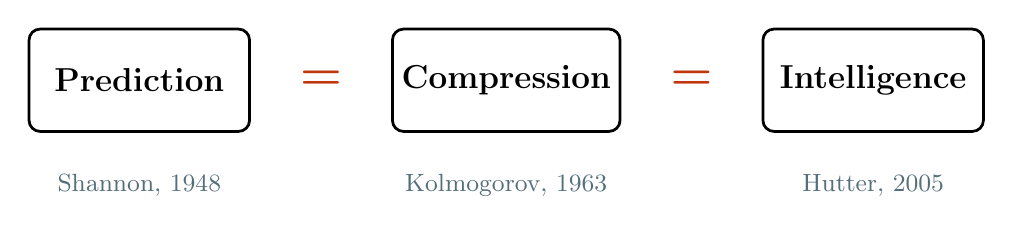
\begin{tikzpicture}[
    box/.style={draw, rounded corners=4pt, minimum width=2.8cm,
                minimum height=1.3cm, align=center, font=\large\bfseries,
                line width=1pt},
    eq/.style={font=\LARGE\bfseries, text=accent}
  ]
  \node[box] (pred) {Prediction};
  \node[eq, right=0.5cm of pred] (e1) {=};
  \node[box, right=0.5cm of e1] (comp) {Compression};
  \node[eq, right=0.5cm of comp] (e2) {=};
  \node[box, right=0.5cm of e2] (intel) {Intelligence};

  \node[below=0.4cm of pred, font=\small\color{muted}] {Shannon, 1948};
  \node[below=0.4cm of comp, font=\small\color{muted}] {Kolmogorov, 1963};
  \node[below=0.4cm of intel, font=\small\color{muted}] {Hutter, 2005};
\end{tikzpicture}
\end{center}

\vspace{0.8em}

\small
\textbf{Shannon:}~Optimal coding length = $-\log_2 p(x_t \mid x_{<t})$.\\
Predict well $\Leftrightarrow$ compress well.

\vspace{0.3em}
\textbf{Hutter/Solomonoff:}~The \emph{perfect} compressor is the most
intelligent possible agent (AIXI).

\note{Claude Shannon proved in 1948 that prediction and compression are two
sides of the same coin. If you can predict the next symbol accurately, you
can assign it a short code --- that is compression. Decades later, Marcus
Hutter formalised the other end: the theoretically perfect compressor would
be the most generally intelligent agent possible. This chain --- prediction
equals compression equals intelligence --- is not a metaphor. It is a
mathematical identity \cite{shannon1948, hutter2005}.}
\end{frame}

% ---------- A3: THE SHOCKING RESULT ----------
\begin{frame}{A Blind Oracle That Sees}

\begin{center}
\begin{tikzpicture}[
    bar/.style={fill=mDarkTeal, minimum width=1cm},
    barh/.style={fill=accent, minimum width=1cm},
    label/.style={font=\footnotesize, anchor=north},
  ]
  % Image compression
  \node[font=\large\bfseries] at (0, 4.5) {Image Compression};
  \draw[bar]  ($(0,0) + (-1.8, 0)$) rectangle ++(1, 3.5);
  \draw[barh] ($(0,0) + (-0.4, 0)$) rectangle ++(1, 2.6);
  \node[label] at (-1.3, -0.1) {PNG};
  \node[label] at (0.1, -0.1) {\textbf{Chinchilla}};
  \node[font=\small, anchor=south] at (-1.3, 3.5) {58.5\%};
  \node[font=\small, anchor=south, text=accent] at (0.1, 2.6) {43.4\%};

  % Audio compression
  \node[font=\large\bfseries] at (6, 4.5) {Audio Compression};
  \draw[bar]  ($(6,0) + (-1.8, 0)$) rectangle ++(1, 1.8);
  \draw[barh] ($(6,0) + (-0.4, 0)$) rectangle ++(1, 1.0);
  \node[label] at (4.7, -0.1) {FLAC};
  \node[label] at (6.1, -0.1) {\textbf{Chinchilla}};
  \node[font=\small, anchor=south] at (4.7, 1.8) {30.3\%};
  \node[font=\small, anchor=south, text=accent] at (6.1, 1.0) {16.4\%};

  % Caption
  \node[font=\small, text=muted, align=center] at (3, -0.9)
    {Compression ratios (lower = better).  Chinchilla 70B was trained
     \emph{only} on text.\\
     D\'{e}letang et al., ``Language Modeling Is Compression,'' ICLR 2024};
\end{tikzpicture}
\end{center}

\note{This is the result that should keep you up at night. Chinchilla 70B is a
text model --- it has never seen a photograph or heard a sound. Yet it
compresses images better than PNG and audio better than FLAC, algorithms
designed specifically for those domains. How? Because next-token prediction
forced it to learn something \emph{universal} about the structure of data
itself \cite{deletang2024}.}
\end{frame}

% ---------- A4: THE IMPLICATION ----------
\begin{frame}{}

\begin{center}
\Large
If compression \textbf{is} understanding,\\[0.5em]
and LLMs are the best compressors\\
we have ever built\ldots

\vspace{1.2em}
\large\color{muted}
\ldots then ``stochastic parrot'' is not just wrong.\\
\emph{It is incoherent.}

\vspace{1.5em}
\normalsize\color{black}
But is that conclusion too fast?
\end{center}

\note{If we accept the Shannon--Hutter chain, then dismissing LLMs as
``stochastic parrots'' is like dismissing a zip file as ``mere bit
shuffling.'' The compression IS the understanding. But this is a strong
claim, and there are reasons to hesitate. We will return to those
reasons in Topic~C. First, let us see where else this thread leads.}
\end{frame}

% ============================================================================
%   TRANSITION A → B
% ============================================================================
\begin{frame}{}

\begin{center}
\large\color{muted}
If prediction captures universal structure\ldots

\vspace{1em}
\Large\color{black}
\textbf{Do all learners converge on the same picture of reality?}
\end{center}

\note{We have established that prediction, compression, and intelligence may
be the same thing. Now a startling empirical question: if every powerful
model is compressing reality, do they all arrive at the same compressed
representation? The answer, increasingly, appears to be \emph{yes}.}
\end{frame}

% ============================================================================
%   TOPIC B: THE PLATONIC REPRESENTATION HYPOTHESIS
% ============================================================================

% ---------- B1: PLATO'S CAVE ----------
\begin{frame}{Plato's Cave, 2,400 Years Later}

\begin{center}
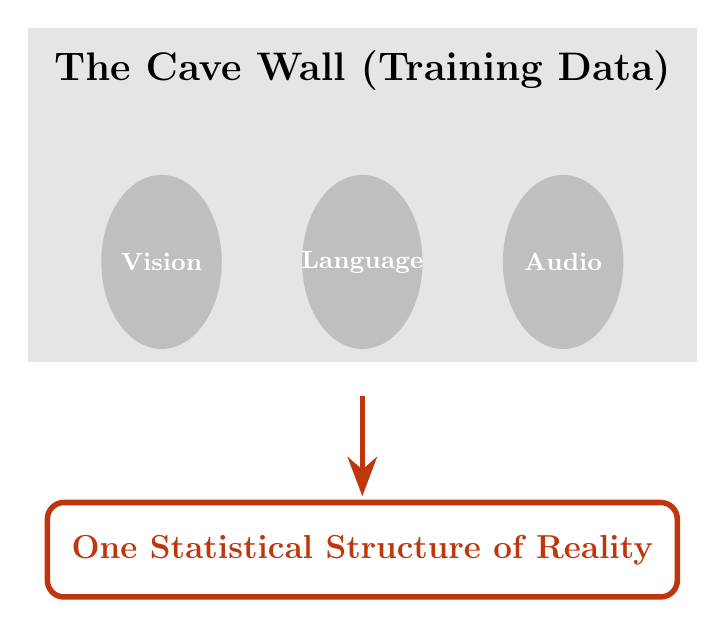
\begin{tikzpicture}[scale=0.85]
  % Cave wall
  \fill[gray!20] (-5, -1) rectangle (5, 4);
  \node[font=\Large\bfseries, anchor=north] at (0, 3.8) {The Cave Wall (Training Data)};

  % Shadows
  \foreach \x/\lbl in {-3/Vision, 0/Language, 3/Audio} {
    \fill[gray!50] (\x, 0.5) ellipse (0.9 and 1.3);
    \node[font=\small\bfseries, white] at (\x, 0.5) {\lbl};
  }

  % Arrow to reality
  \draw[-{Stealth[length=5mm]}, line width=2pt, accent]
    (0, -1.5) -- (0, -3);

  % Platonic form
  \node[draw, accent, line width=2pt, rounded corners=6pt,
        minimum width=8cm, minimum height=1.2cm,
        font=\large\bfseries, text=accent] at (0, -3.8)
    {One Statistical Structure of Reality};
\end{tikzpicture}
\end{center}

\vspace{0.3em}
\centering\small
\emph{Different models, data, architectures $\longrightarrow$ converging representations.}\\
Huh et al., ``The Platonic Representation Hypothesis,'' ICML 2024

\note{Plato argued that behind the messy world of appearances lies a realm of
perfect Forms. Twenty-four centuries later, a team at MIT showed that AI
models --- trained by different companies, on different data, with different
architectures --- are converging on increasingly similar internal
representations as they scale up. Plato, it turns out, may have been
describing neural networks \cite{huh2024}.}
\end{frame}

% ---------- B2: OTHELLO-GPT ----------
\begin{frame}{The Model That Discovered a World}

\begin{center}
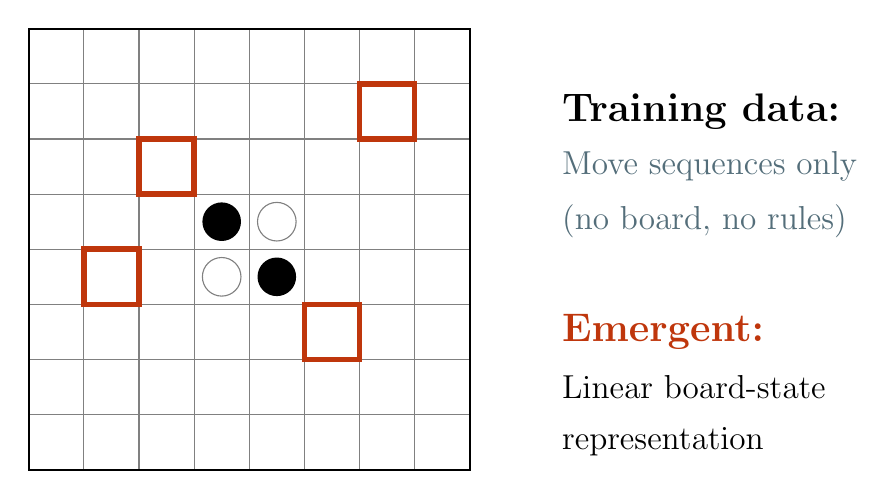
\begin{tikzpicture}[scale=0.7]
  % Board grid
  \draw[step=1, gray, thin] (0,0) grid (8,8);
  \draw[thick] (0,0) rectangle (8,8);

  % Some pieces to suggest Othello
  \foreach \x/\y in {3/3, 4/4} {
    \fill[white] (\x+0.5, \y+0.5) circle (0.35);
    \draw[gray] (\x+0.5, \y+0.5) circle (0.35);
  }
  \foreach \x/\y in {3/4, 4/3} {
    \fill[black] (\x+0.5, \y+0.5) circle (0.35);
  }

  % Highlight emergent neurons
  \foreach \x/\y in {2/5, 5/2, 6/6, 1/3} {
    \draw[accent, line width=2pt] (\x, \y) rectangle ++(1,1);
  }

  % Labels
  \node[font=\Large\bfseries, anchor=west] at (9.5, 6.5)
    {Training data:};
  \node[font=\large, anchor=west, text=muted] at (9.5, 5.5)
    {Move sequences only};
  \node[font=\large, anchor=west, text=muted] at (9.5, 4.5)
    {(no board, no rules)};

  \node[font=\Large\bfseries, anchor=west, text=accent] at (9.5, 2.5)
    {Emergent:};
  \node[font=\large, anchor=west] at (9.5, 1.5)
    {Linear board-state};
  \node[font=\large, anchor=west] at (9.5, 0.5)
    {representation};
\end{tikzpicture}
\end{center}

\vspace{0.3em}
\centering\small
Li et al., ``Emergent World Representations,'' ICLR 2023;\\
Nanda, ``Linear Emergent World Representation,'' 2023

\note{A model called Othello-GPT was trained only on sequences of Othello
moves --- raw coordinate pairs. It was never told a board exists, never
shown the rules. Yet researchers found, inside its weights, a clean
linear representation of the full board state. The model \emph{inferred
the existence of a world it was never shown}. And this representation
was not a tangled mess --- it was geometrically clean, linearly
decodable \cite{li2023, nanda2023}.}
\end{frame}

% ---------- B3: SPACE AND TIME NEURONS ----------
\begin{frame}{Space and Time, Inside a Language Model}

\begin{center}
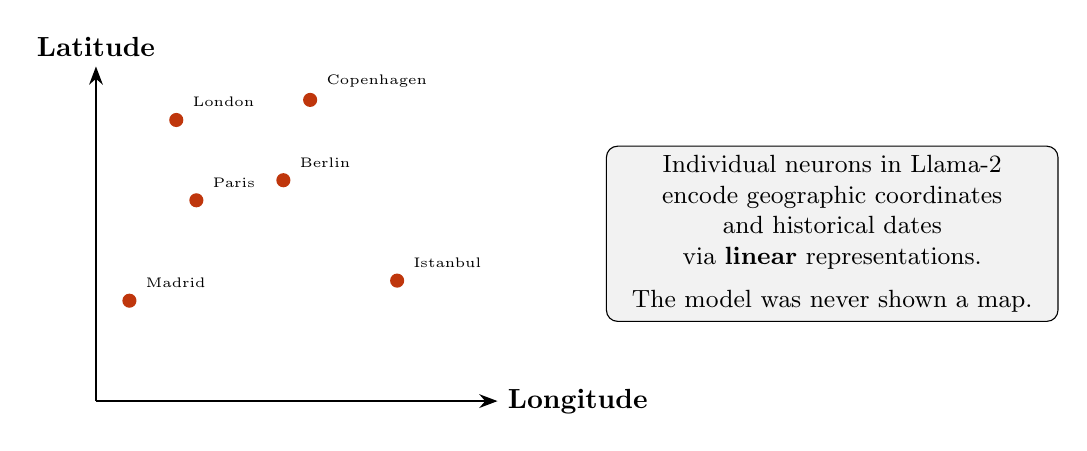
\begin{tikzpicture}[scale=0.85]
  % Space axis
  \draw[-{Stealth}, thick] (0,0) -- (6,0) node[right, font=\bfseries] {Longitude};
  \draw[-{Stealth}, thick] (0,0) -- (0,5) node[above, font=\bfseries] {Latitude};

  % Scattered city dots
  \foreach \x/\y/\lbl in {1.2/4.2/London, 1.5/3.0/Paris, 2.8/3.3/Berlin,
    4.5/1.8/Istanbul, 0.5/1.5/Madrid, 3.2/4.5/Copenhagen} {
    \fill[accent] (\x, \y) circle (3pt);
    \node[font=\tiny, anchor=south west] at (\x+0.1, \y+0.05) {\lbl};
  }

  % Caption box
  \node[draw, rounded corners, fill=gray!10, align=center,
        font=\small, text width=5.5cm] at (11, 2.5)
    {Individual neurons in Llama-2 \\encode geographic coordinates\\
     and historical dates\\via \textbf{linear} representations.\\[0.5em]
     The model was never shown a map.};
\end{tikzpicture}
\end{center}

\vspace{0.3em}
\centering\small
Gurnee \& Tegmark, ``Language Models Represent Space and Time,'' ICLR 2024

\note{Gurnee and Tegmark probed the internals of Llama-2 and found individual
neurons that fire in proportion to geographic longitude and latitude, and
others that encode historical dates on a linear timeline. The model was
trained on text. It was never shown a map or a calendar. Yet it built
spatial and temporal coordinate systems from pure language
\cite{gurnee2024}. This is convergence at the level of individual neurons.}
\end{frame}

% ---------- B4: THE COMMODITY QUESTION ----------
\begin{frame}{}

\begin{center}
\Large
If all foundation models converge\\
on the same representation of reality\ldots

\vspace{1em}
\large\color{muted}
\ldots does it matter which one you buy?

\vspace{1em}
\normalsize\color{black}
Or is intelligence a commodity --- like electricity ---\\
where the only question is \alert{price}?
\end{center}

\note{This is the business implication that should give every AI startup pause.
If the Platonic Representation Hypothesis is correct, then differentiation
between foundation models shrinks as scale increases. The endgame may be
commoditised intelligence, competing on cost, speed, and reliability ---
not on unique ``understanding.'' Of course, we are not there yet, and the
hypothesis remains debated.}
\end{frame}

% ============================================================================
%   TRANSITION B → C
% ============================================================================
\begin{frame}{}

\begin{center}
\large\color{muted}
Models that predict, compress, and converge on reality\ldots

\vspace{1em}
\Large\color{black}
\textbf{Do they \emph{understand}?}
\end{center}

\note{We have now seen two extraordinary claims: that compression is
understanding, and that all models converge on the same picture of
reality. The obvious question follows: do these systems actually
\emph{understand} anything? This question is 45 years old, and it
starts with a philosopher and a room full of Chinese characters.}
\end{frame}

% ============================================================================
%   TOPIC C: THE CHINESE ROOM, 45 YEARS LATER
% ============================================================================

% ---------- C1: THE CHINESE ROOM ----------
\begin{frame}{Searle's Chinese Room (1980)}

\begin{center}
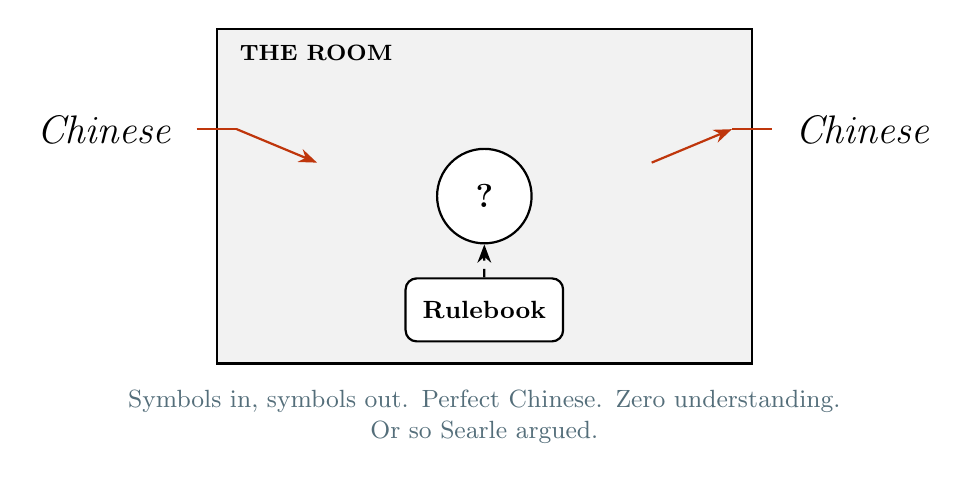
\begin{tikzpicture}[scale=0.85]
  % Room
  \draw[thick, fill=gray!10] (0,0) rectangle (8, 5);
  \node[font=\footnotesize\bfseries, anchor=north west] at (0.2, 4.9) {THE ROOM};

  % Person
  \node[draw, circle, minimum size=1.2cm, thick, fill=white,
        font=\large] (person) at (4, 2.5) {\textbf{?}};

  % Rulebook
  \node[draw, thick, fill=white, rounded corners, minimum width=2cm,
        minimum height=0.8cm, font=\small\bfseries] (book) at (4, 0.8)
    {Rulebook};
  \draw[-{Stealth}, thick, dashed] (book) -- (person);

  % Input slot
  \draw[thick, accent] (-0.3, 3.5) -- (0.3, 3.5);
  \node[font=\Large, anchor=east] at (-0.5, 3.5) {\textit{Chinese}};
  \draw[-{Stealth}, thick, accent] (0.3, 3.5) -- (1.5, 3.0);

  % Output slot
  \draw[thick, accent] (7.7, 3.5) -- (8.3, 3.5);
  \node[font=\Large, anchor=west] at (8.5, 3.5) {\textit{Chinese}};
  \draw[-{Stealth}, thick, accent] (6.5, 3.0) -- (7.7, 3.5);

  % Caption
  \node[font=\small, text=muted, align=center, text width=10cm]
    at (4, -0.8)
    {Symbols in, symbols out. Perfect Chinese. Zero understanding.\\
     Or so Searle argued.};
\end{tikzpicture}
\end{center}

\note{In 1980, philosopher John Searle proposed his most famous thought
experiment. A person sits in a room, receives Chinese characters through
a slot, looks them up in an enormous rulebook, and pushes the ``correct''
Chinese characters back out. To the outside world, the room speaks perfect
Chinese. But the person inside understands \emph{nothing}. Searle's
conclusion: syntax is not semantics; computation alone cannot produce
understanding \cite{searle1980}. Now --- what if the rulebook is 175
billion parameters large?}
\end{frame}

% ---------- C2: THE EVIDENCE FOR ----------
\begin{frame}{Evidence \emph{For} Understanding}

\begin{center}
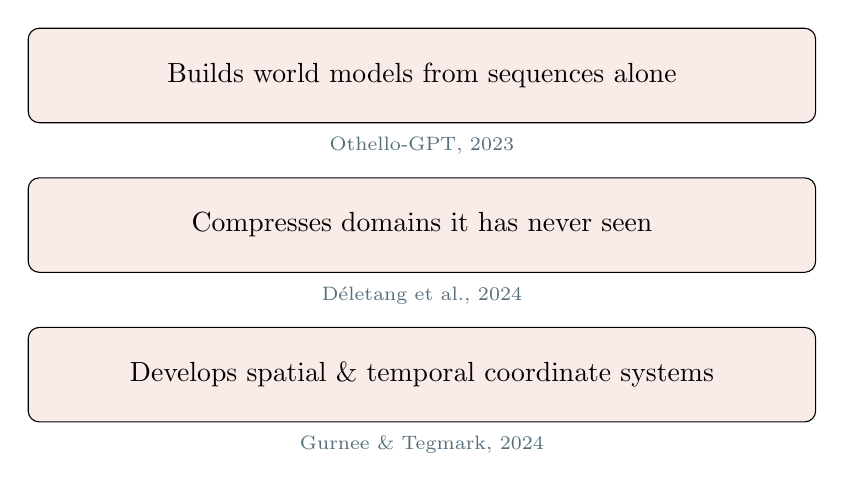
\begin{tikzpicture}[
    evidence/.style={draw, rounded corners=4pt, fill=accent!10,
                     minimum width=10cm, minimum height=1.2cm,
                     align=center, font=\normalsize},
    ref/.style={font=\scriptsize, text=muted}
  ]
  \node[evidence] (e1) at (0, 3.8)
    {Builds world models from sequences alone};
  \node[ref, below=0.05cm of e1] {Othello-GPT, 2023};

  \node[evidence] (e2) at (0, 1.9)
    {Compresses domains it has never seen};
  \node[ref, below=0.05cm of e2] {D\'{e}letang et al., 2024};

  \node[evidence] (e3) at (0, 0.0)
    {Develops spatial \& temporal coordinate systems};
  \node[ref, below=0.05cm of e3] {Gurnee \& Tegmark, 2024};
\end{tikzpicture}
\end{center}

\vspace{0.5em}
\centering
Each finding erodes Searle's premise:\\
\emph{these are not ``mere symbol manipulations.''}

\note{Let us stack up what we have seen today. The model builds world models
from sequences it was never told contain a world. It compresses images and
audio it has never encountered. It develops spatial and temporal coordinate
systems from text alone. Each of these findings erodes the core premise of
the Chinese Room: that what is happening inside is ``mere symbol
manipulation'' with no connection to meaning.}
\end{frame}

% ---------- C3: THE EVIDENCE AGAINST ----------
\begin{frame}{Evidence \emph{Against} Understanding}

\begin{center}
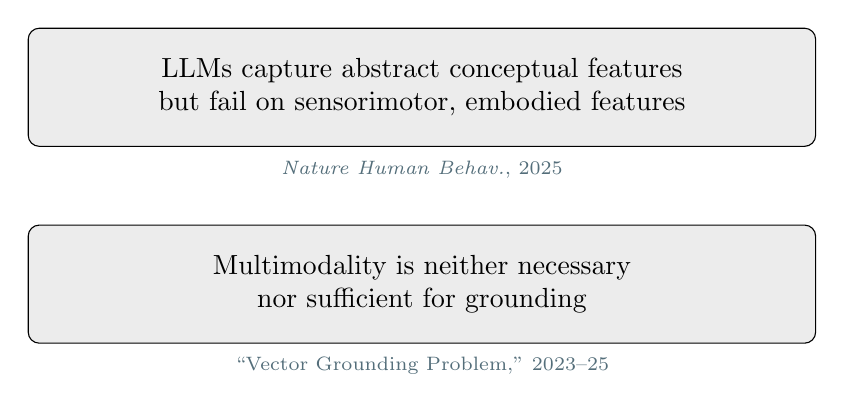
\begin{tikzpicture}[
    evidence/.style={draw, rounded corners=4pt, fill=gray!15,
                     minimum width=10cm, minimum height=1.5cm,
                     align=center, font=\normalsize},
    ref/.style={font=\scriptsize, text=muted}
  ]
  \node[evidence] (e1) at (0, 3.0)
    {LLMs capture abstract conceptual features\\
     but \alert{fail on sensorimotor, embodied features}};
  \node[ref, below=0.05cm of e1] {\emph{Nature Human Behav.}, 2025};

  \node[evidence] (e2) at (0, 0.5)
    {Multimodality is neither necessary\\
     nor sufficient for grounding};
  \node[ref, below=0.05cm of e2] {``Vector Grounding Problem,'' 2023--25};
\end{tikzpicture}
\end{center}

\vspace{0.5em}
\centering
LLMs know that lemons are yellow and sour.\\
They do not know what it \emph{feels like} to bite one.

\note{But the picture is not clean. A 2025 study in Nature Human Behaviour
showed that LLMs recover abstract and linguistic features of human concepts
--- but fail systematically on sensorimotor and embodied features. They know
lemons are yellow; they do not know what it feels like to hold one, to smell
one, to wince at the sourness. And adding images does not solve this: the
``Vector Grounding Problem'' shows that multimodality is neither necessary
nor sufficient for genuine grounding \cite{nature2025, vectorgrounding2023}.}
\end{frame}

% ---------- C4: THE HONEST ANSWER ----------
\begin{frame}{}

\begin{center}
\LARGE
We cannot say whether LLMs understand.

\vspace{1em}
\large\color{muted}
Not because we lack data.\\[0.4em]
Because we lack a \alert{definition}.

\vspace{1.5em}
\normalsize\color{black}
This is not evasion. It is the actual state of knowledge.
\end{center}

\note{Here is the uncomfortable conclusion. After 45 years of debating the
Chinese Room, the bottleneck is not empirical --- we have mountains of
evidence. The bottleneck is conceptual. We do not possess a rigorous,
agreed-upon definition of ``understanding'' that would let us answer
the question. This is not evasion or false modesty. It is the honest
state of the field, acknowledged by philosophers and AI researchers
alike \cite{inquiry2025}.}
\end{frame}

% ============================================================================
%   DISCUSSION & CLOSE
% ============================================================================

% ---------- DISCUSSION ----------
\begin{frame}{Discussion: Three Questions for the Room}

\begin{enumerate}
\Large
\item If compression \emph{is} understanding, should we treat\\
      LLMs as genuine ``knowers'' --- or not?

\vspace{0.8em}
\item If all models converge on one representation,\\
      what is your company's AI moat?

\vspace{0.8em}
\item If we cannot define ``understanding,'' how do\\
      you decide whether to trust a machine\\
      with a critical decision?
\end{enumerate}

\note{These are the three questions I would like you to sit with.
The first is philosophical but has regulatory implications. The second is
a direct business strategy question. The third is the one you are already
facing, whether you realise it or not --- every deployment of an LLM in
your organisation is an implicit bet on a definition of understanding
that does not yet exist.}
\end{frame}

% ---------- READING LIST ----------
\begin{frame}{Further Reading}

\footnotesize
\begin{description}
  \item[Prediction = Compression]~\\
    D\'{e}letang et al., ``Language Modeling Is Compression'' (ICLR 2024)\\
    Hutter, \emph{Universal Artificial Intelligence} (Springer, 2005)

  \vspace{0.4em}
  \item[Platonic Representations]~\\
    Huh et al., ``The Platonic Representation Hypothesis'' (ICML 2024)\\
    Gurnee \& Tegmark, ``LMs Represent Space and Time'' (ICLR 2024)

  \vspace{0.4em}
  \item[The Chinese Room Today]~\\
    Searle, ``Minds, Brains, and Programs'' (BBS, 1980)\\
    Nature Human Behaviour, ``LLMs without grounding\ldots'' (2025)

  \vspace{0.4em}
  \item[Popular Accounts]~\\
    Quanta Magazine, ``The Converging World of AI'' (Jan 2026)
\end{description}

\note{These are the key references. For those who want just one paper from
each topic: D\'{e}letang et al.\ for compression, Huh et al.\ for the
Platonic Representation Hypothesis, and the 2025 Nature Human Behaviour
paper for the most nuanced empirical answer to the understanding question.}
\end{frame}

% ---------- CLOSING ----------
\begin{frame}{}

\begin{center}
\Large
\emph{``The question is not whether machines think.}\\[0.5em]
\emph{The question is whether we know\\
what \textbf{we} mean by `thinking.'\,''}

\vspace{2em}
\normalsize\color{muted}
Philosophy is not the bottleneck you expected.\\
But it may be the bottleneck that matters most.
\end{center}

\note{I will leave you with this thought. The most important obstacle to
deploying AI wisely is not technical --- it is conceptual. Until we
clarify what we mean by understanding, knowledge, and intelligence,
we will keep arguing past each other. And in the meantime, you are
making billion-dollar bets on implicit answers to questions that
philosophers have not yet resolved. Thank you.}
\end{frame}

% ============================================================================
%   BIBLIOGRAPHY
% ============================================================================
\begin{frame}[allowframebreaks]{References}
\scriptsize\raggedright
\begin{thebibliography}{99}

\bibitem{shannon1948}
C.~E. Shannon,
``A Mathematical Theory of Communication,''
\emph{Bell System Technical Journal}, vol.~27, pp.~379--423, 1948.

\bibitem{hutter2005}
M.~Hutter,
\emph{Universal Artificial Intelligence: Sequential Decisions Based on
Algorithmic Probability},
Springer, 2005.

\bibitem{deletang2024}
G.~D\'{e}letang, A.~Ruoss, P.-A.~Duquenne, E.~Catt, T.~Genewein, C.~Mattern,
J.~Grau-Moya, L.~K.~Wenliang, M.~Aitchison, L.~Orseau, M.~Hassabis, and
S.~Legg,
``Language Modeling Is Compression,''
\emph{Proc.\ ICLR}, 2024.  arXiv:2309.10668.

\bibitem{kaplan2020}
J.~Kaplan, S.~McCandlish, T.~Henighan, T.~B.~Brown, B.~Chess, R.~Child,
S.~Gray, A.~Radford, J.~Wu, and D.~Amodei,
``Scaling Laws for Neural Language Models,''
arXiv:2001.08361, 2020.

\bibitem{huh2024}
M.~Huh, B.~Cheung, T.~Wang, and P.~Isola,
``Position: The Platonic Representation Hypothesis,''
\emph{Proc.\ ICML}, 2024.  arXiv:2405.07987.

\bibitem{gurnee2024}
W.~Gurnee and M.~Tegmark,
``Language Models Represent Space and Time,''
\emph{Proc.\ ICLR}, 2024.

\bibitem{li2023}
K.~Li, A.~K.~Hopkins, D.~Bau, F.~Vi\'{e}gas, H.~Pfister, and M.~Wattenberg,
``Emergent World Representations: Exploring a Sequence Model Trained on a
Synthetic Task,''
\emph{Proc.\ ICLR}, 2023.

\bibitem{nanda2023}
N.~Nanda, ``Actually, Othello-GPT Has A Linear Emergent World Representation,''
Blog post, 2023.

\bibitem{searle1980}
J.~R. Searle,
``Minds, Brains, and Programs,''
\emph{Behavioral and Brain Sciences}, vol.~3, no.~3, pp.~417--424, 1980.

\bibitem{nature2025}
``Large language models without grounding recover non-sensorimotor but not
sensorimotor features of human concepts,''
\emph{Nature Human Behaviour}, 2025.

\bibitem{inquiry2025}
``LLMs, Turing Tests and Chinese Rooms,''
\emph{Inquiry}, 2025.

\bibitem{vectorgrounding2023}
``The Vector Grounding Problem,''
arXiv:2304.01481, 2023 (updated 2025).

\end{thebibliography}
\end{frame}

\end{document}
